\chapter{Discussion}
Please tell more about conclusion and how to the next work of this study.

\section{Andri Fajar Sunandhar / 1164065}
\subsection{Teori}
\begin{enumerate}

\item Jelaskan kenapa file teks harus dilakukan tokenizer, dilengkapi dengan ilustrasi atau gambar.
	\par Tokenizer adalah untuk membuat vektor dari teks. File teks harus dilakukan tokenizer karena dengan memfungsikan tokenizer teks dapat divektorkan. Maka dari itu harus menginport tokenizer dari keras, sehingga teks yang telah telah divektorkan tersebut dapat terbaca pada Machine Learning. Ilustrasinya bisa dilihat pada gambar \ref{no1}.
	\begin{figure}[ht]
	\centerline{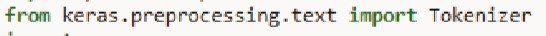
\includegraphics[width=0.5\textwidth]{figures/chapter7/no1.jpg}}
	\caption{Tokenizer}
	\label{no1}
	\end{figure}

\item Menjelaskan konsep dasar K-Fold Cross Validation
	\lstinputlisting[firstline=8, lastline=20]{src/chapter7/A2.py}
	\par Penjelasan kode listingg :
	\begin{enumerate}
	\item Membuat variabel kfold yang memanggil fungsi StratifiedKFold. StratifiedKFold itu sendiri ialah variasi Kfold yang mengembalikan lipatan bertingkat. Yang dimana pada kode program tersebut jumlah lipatannya adalah 5 atau dibagi menjadi 5 bagian.
	\item Membuat variabel split yang mempresentasikan variabel kfold untuk dibagi berdasarkan class.
	\end{enumerate}
	
	\par Berikut adalah gambar  \ref{no2} ilustrasi dari kosep dasar kfold.
		\begin{figure}[!hbtp]
		\centering
		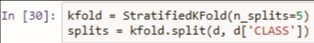
\includegraphics[scale=0.4]{figures/chapter7/no2.jpg}
		\caption{StratifiedKFold}
		\label{no2}
		\end{figure}

\item Jelaskan apa maksudnya kode program for train, test in splits, dilengkapi dengan ilustrasi atau gambar
	\par Maksudnya yaitu untuk menguji apakah setiap data pada dataset sudah di split dan tidak terjadi penumpukan. Yang dimana maksudnya di setiap class tidak akan muncul id yang sama. Ilustrasinya misalkan kita memiliki 5 jam tangan dengan model yang berbeda. Kemudian kita bagikan jam tersebut kepada teman, tentunya teman tersebut yang menerima jam tangan itu tidak memiliki jam yang sama modelnya.
 

\item Menjelaskan maksud kode program
	\lstinputlisting[firstline=8, lastline=20]{src/chapter7/A4.py}
	\par Dari kode program tersebut dapat dijelaskan bahwa membuat fungsi train dan test dengan menggunakan dataset yang hanya diambil kolom 'CONTENT' saja. iloc berfingsi sebagai pengindeksan posisi menggunakan integer.
	
	\par Berikut ilustrasi dari kode program tersebut, perhatikan gambar \ref{no4}.
		\begin{figure}[!hbtp]
		\centering
		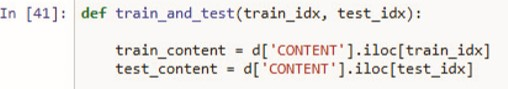
\includegraphics[scale=0.4]{figures/chapter7/no4.jpg}
		\caption{Ilustrasi Kode Program No.4}
		\label{no4}
		\end{figure}

\item Apa Maksud Dari Fungsi Tokenizer = Tokenizer(num words=2000) Dan Tokenizer.fit on texts(train content), Dilengkapi Dengan Ilustrasi Gambar
	\lstinputlisting[firstline=8, lastline=20]{src/chapter7/A5.py}
		
	\par Dari kode program  membuat variabel tokenizer untuk memanggil fungsi tokenizer agar dapat dilakukan vektorisasi dari kata. Dimana pada kode program pada baris pertama menggunakan 2000 kata atau 2000 kolom.
	
	
	\par Berikut adalah gambar  \ref{no5}  ilustrasi dari fungsi pada kode program tersebut.
	
		\begin{figure}[!hbtp]
		\centering
		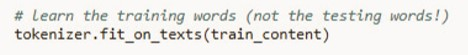
\includegraphics[scale=0.4]{figures/chapter7/no5.jpg}
		\caption{fungsi tokenizer}
		\label{no5}
		\end{figure}

\item  Apa Maksud Dari Fungsi d train inputs = tokenizer.texts to matrix(train content, mode=’tfidf ’) dan d test inputs = tokenizer.texts to matrix(test content, mode=’tfidf ’), Dilengkapi Dengan Ilustrasi Kode Dan Atau Gambar

\item Apa Maksud Dari Fungsi d train inputs = d train inputs/np.amax(np.absolute(d\_train) :

\item Jelaskan apa maksud dari fungsi d\_train\_outputs dan d\_test\_outputs, dilengkapi dengan ilustrasi atau gambar.

\item Jelaskan apa maksud dari fungsi di listing 7.2 , Gambarkan ilustrasi Neural Networknya.

\item Jelaskan apa maksud dari fungsi di listing 7.3 .

\item Jelaskan apa itu Deep Learning.
	\par Deep Learning merupakan cabang dari Machine Learning atau bagian keluarga yang lebih luas dari method machine learning berdasarkan pada representasi data pembelajaran. Deep Learning menggunakan Deep Neural Network dalam menyelesaikan suatu masalah yang terjadi pada Machine Learning.

\item Jelaskan apa itu Deep Neural Network, dan apa bedanya dengan Deep Learning.
	\par Deep Neural Network atau DNN merupakan algoritma yang berbasis neural network yang digunakan untuk mengambil keputusan. Yang membedakan Deep Learning dengan  Deep Neural Network (DNN) adalah DNN merupakan algoritma yang digunakan pada Deep Learning, sedangkan Deep Learning merupakan model yang menggunakan algoritma DNN.

\item Jelaskan dengan ilustrasi gambar langkah per langkah bagaimana perhitungan algoritma konvolusi dengan ukuran stide (NPM mod 3 + 1) x (NPM mod 3 + 1) yang terdapat max pooling !

	\begin{itemize}
		\item Pertama tentukan nilai (x,y) dan (x1,y1)
		\item Nilai tersebut dibuat kedalam bentuk matrix
		\item Jika sudah berbentuk matrix lakukan perkalian antar baris dan deret
		\item Hasil perkalian tersebut dijumlahkan sehingga akan menghasilkan nilai matrix (3x3)
	\end{itemize}

	\subitem Untuk ilustrasi dapat dilihat pada figure \ref{no13}

	\begin{figure}[!htbp!]
		\centerline{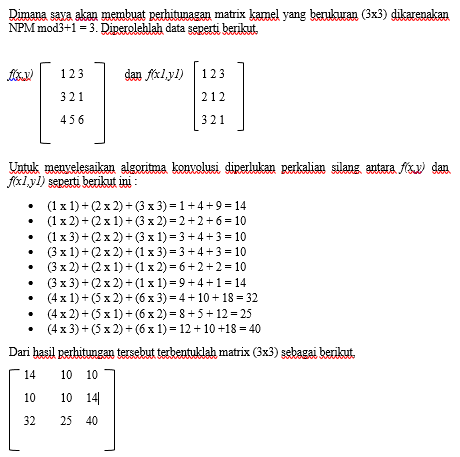
\includegraphics[width=0.5\textwidth]{figures/Chapter7/no13.png}}
		\caption{Algoritma Konvolusi Dengan Matrix (3x3).}
		\label{no13}
	\end{figure}	

\end{enumerate}





\subsection{Praktek}
\begin{enumerate}
\item Jelaskan kode program pada blok \# In [1]. 

\item Jelaskan kode program pada blok \# In [2] .

\item Jelaskan kode program pada blok \# In [3] .

\item Jelaskan kode program pada blok \# In [4] .

\item Jelaskan kode program pada blok \# In [5] .

\item Jelaskan kode program pada blok \# In [6] .

\item Jelaskan kode program pada blok \# In [7] .

\item Jelaskan kode program pada blok \# In [8] .

\item Jelaskan kode program pada blok \# In [9] .

\item Jelaskan kode program pada blok \# In [10] .

\item Jelaskan kode program pada blok \# In [11] .

\item Jelaskan kode program pada blok \# In [12] .

\item Jelaskan kode program pada blok \# In [13] .

\item Jelaskan kode program pada blok \# In [14] .

\item Jelaskan kode program pada blok \# In [15] .

\item Jelaskan kode program pada blok \# In [16] .

\item Jelaskan kode program pada blok \# In [17] .

\item Jelaskan kode program pada blok \# In [18] .

\item Jelaskan kode program pada blok \# In [19] .

\item Jelaskan kode program pada blok \# In [20] .


\end{enumerate}


\subsection{Penanganan Error}
Dari praktek pemrograman yang dilakukan di modul ini, error yang kita dapatkan(hasil komputer sendiri) di dokumentasikan dan di selesaikan(nilai 5 per error yang ditangani. Untuk hari kedua):

\begin{enumerate}
	\item skrinsut error
		
		
	\item Tuliskan kode error dan jenis errornya
		\begin{enumerate}
		\item Kode Error  :
			\begin{itemize}
				\item Kode error : 
				\item Jenis error :
			\end{itemize}
		\end{enumerate}

	\item Solusi pemecahan masalah error
		
		
\end{enumerate}